\section{Visualization}~\label{sec: visualization}
\subsection{SFC for HyperGraph}

In the design guidelines proposed by Abdelaal et al.~\cite{abdelaal2022network} in a recent network visualization evaluation study, node-link-based approaches are recommended when:
(1) tasks involve the identification of network clusters, and (2) the network is sparse.
Condition (1) is fulfilled as explained in~\autoref{sec: design_rationale}, and (2) is guaranteed by the main participant extraction process described in~\autoref{sec: participant_extraction}. 
Therefore, we decided to use node-link-based approaches for our system.

Although there are a variety of node-link-based approaches for hypergraph visualization, we find the extra-node representation proposed by Ouvrard et al.~\cite{ouvrard2017hypergraph} most flexible and intuitive.
An extra-node representation improves existing clique-expansion of hypergraphs by adding extra nodes to represent hyperedges. 
The extra-node representation effectively transforms the hypergraph visualization problem into a bipartite graph visualization problem.
After that, any node-link-based graph visualization method can be applied.
In our system, we use the space-filling curve (SFC) layout method to layout the extra-node representation of the hypergraph.
The SFC layout method uses pre-computed clustering to order nodes in a sequence and then applies a space-filling curve on the node sequence to map it to a two-dimensional screen space~\cite{muelder2008sfc}.
SFC approaches are known for their efficiency and aesthetics in visualizing large graphs~\cite{ma2013largegraph}.
Moreover, SFC layouts support progressive disclosure (\textbf{DC2}) organically, as the layout is generated based on the clustering result (\textbf{DC3}).
After the preprocessing and modeling stage described in~\autoref{sec: methodology}, we have two hypergraphs: the article hypergraph $H_A$ and the participant hypergraph $H_P$, each having its hierarchical cluster.
Combining the extra-node representation and SFC layout, we visualize the article hypergraph $H_A$ and the participant hypergraph $H_P$ as two separate SFCs, as shown in~\autoref{fig: sfc}.

Specifically, we divide the layout space into two parts: the peripheral and the center area.
For the peripheral area, we concatenate four generalized Hilbert (Gilbert) curves~\cite{gilbert}.
A Gilbert curve is a generalized version of the Hilbert curve that can traverse any rectangular region in a way similar to the Hilbert Curve.
In~\autoref{fig: gilbert_raw}, the Gilbert curve starts from the lower left (dark blue) and ends at the lower right (dark red).
Through rotation and flipping, the start and end curve points for neighboring Gilbert curves can be concatenated smoothly, as shown in~\autoref{fig: gilbert_concat}.
The use of concatenated Gilbert curves allows us to fill the peripheral space while having the efficiency and aesthetics of SFC layouts.

The curve to be used for the center area is technically unbounded. 
In early prototyping, we found that using the same curve as the peripheral region was confusing for the user, as it was hard to distinguish between the peripheral and center areas.
We decided to use a simple Gosper curve (\autoref{fig: gosper}) to layout the nodes for better aesthetics.
The resulting visualization looks similar to GosperMap~\cite{auber2013gospermap}, but we did not employ the advanced techniques proposed in GosperMap.
The interactions to support the exploration and reorganization of the dataset are the main focus of the system, which are also not limited to any specific curve.

After the curves are generated, we can apply the curves on the node sequences to generate the two-dimensional layout.
We chose to put the article hypergraph in the center area because the articles are the main analysis targets for the user.
Consequently, the participant hypergraph is put in the peripheral area.
\begin{figure}%
    \centering
    \subfloat[\centering One Gilbert curve\label{fig: gilbert_raw}]{{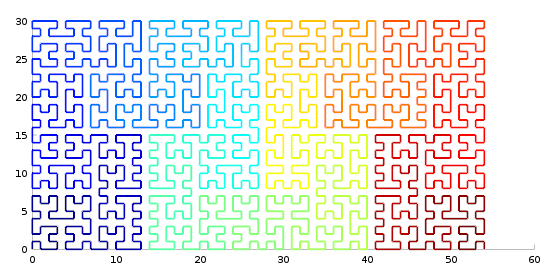
\includegraphics[width=5cm]{gilbert} }}
    \qquad
    \subfloat[\centering Four concatenated Gilbert curves\label{fig: gilbert_concat}]{{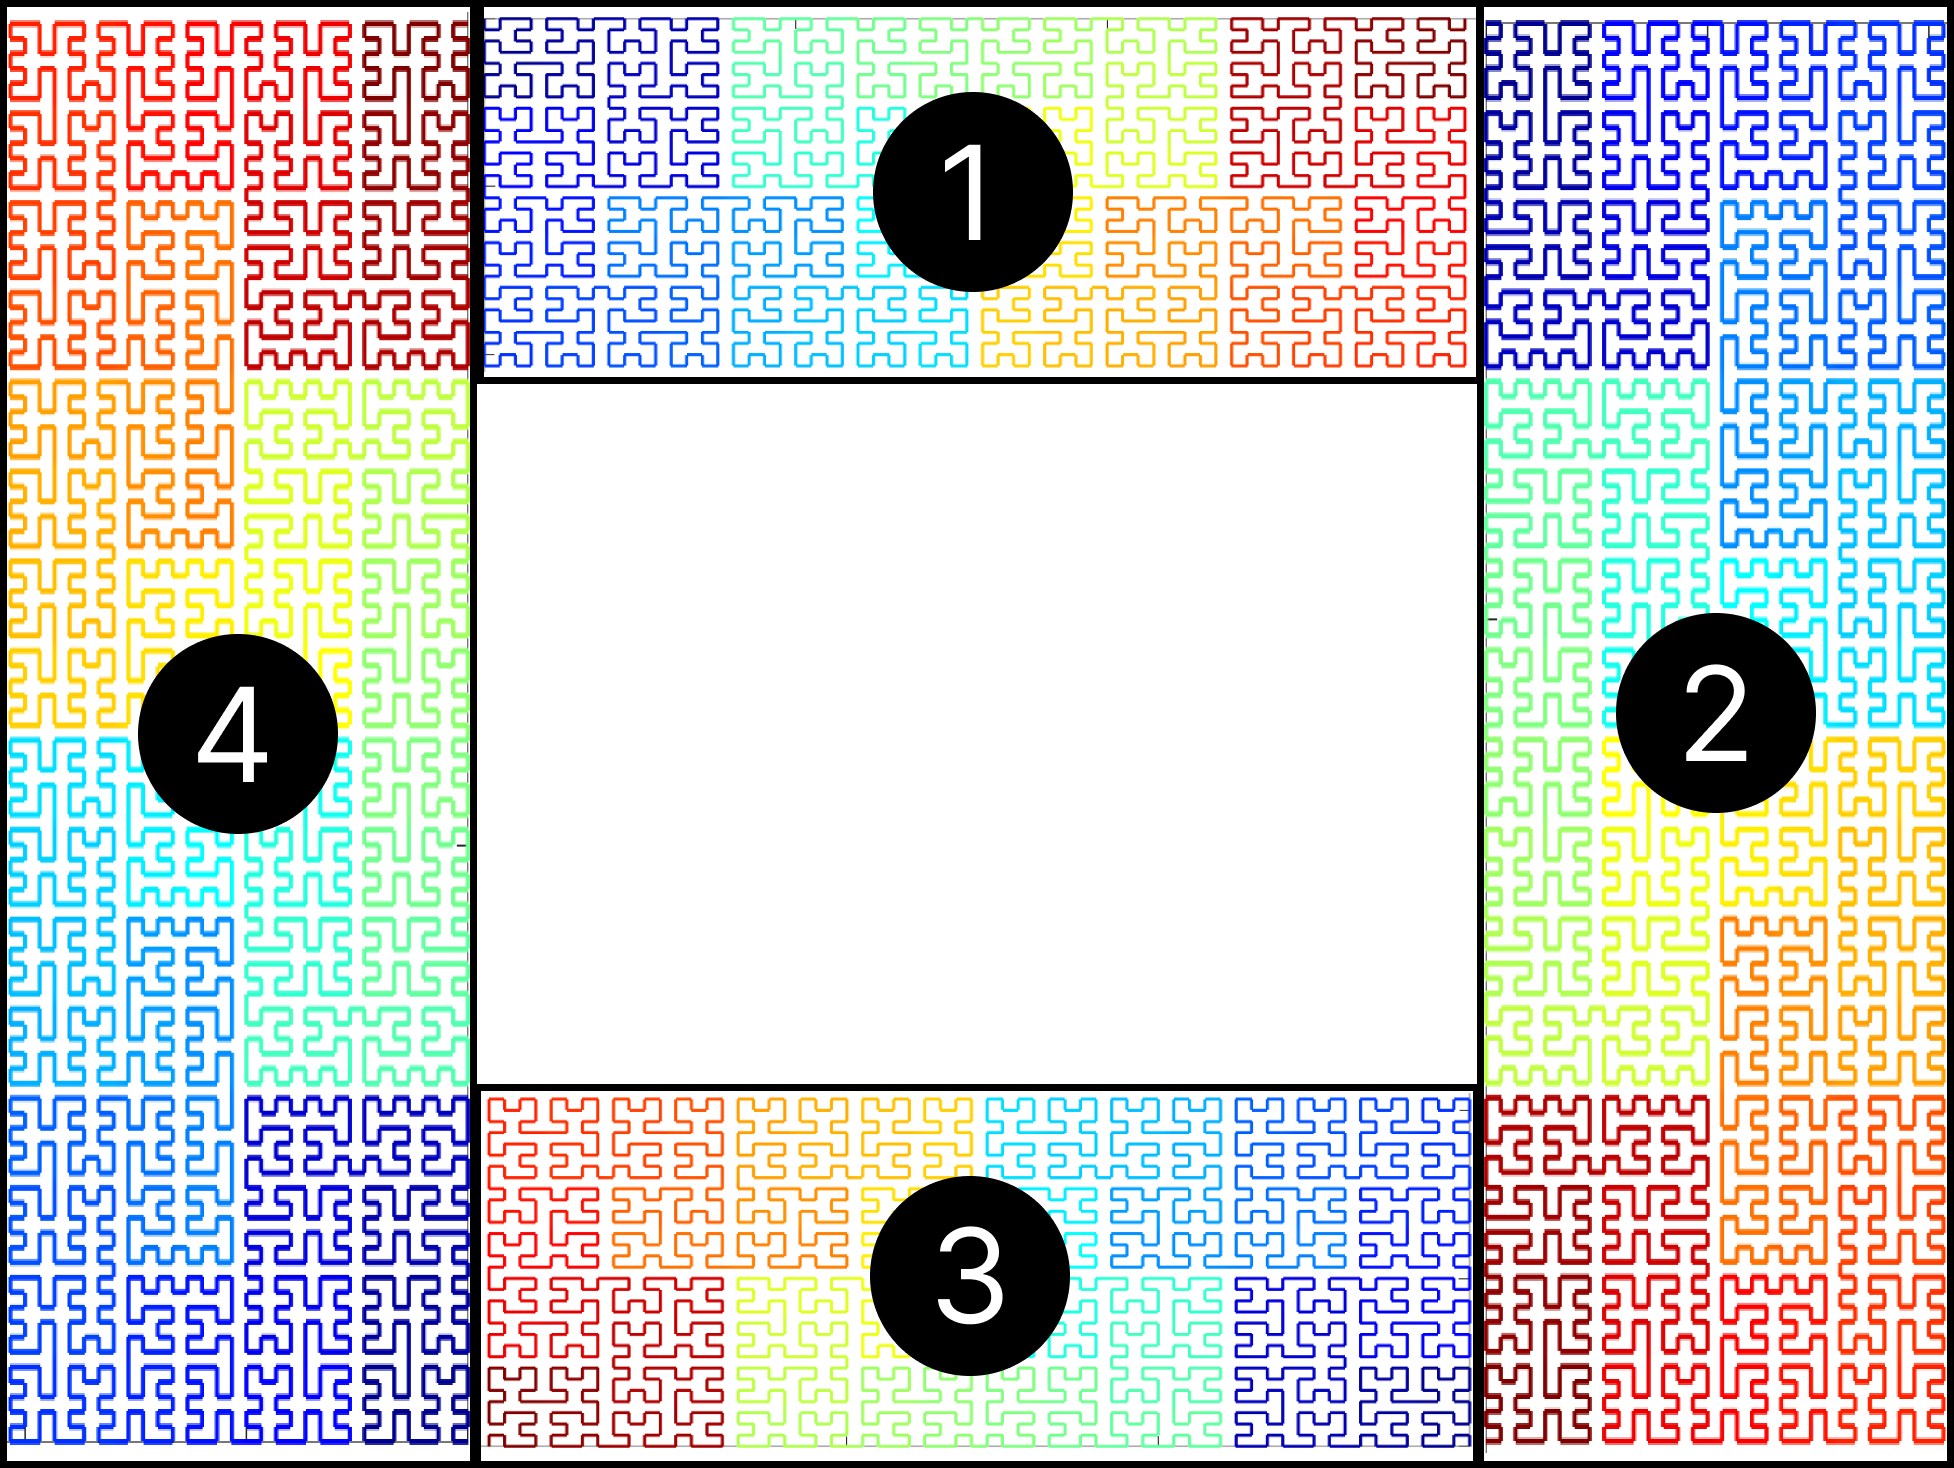
\includegraphics[width=5cm]{concatenated_gilbert} }}%
    \qquad
    \subfloat[\centering An order-4 Gosper curve\label{fig: gosper}]{{
\includegraphics[width=5cm]{gosper} }}%
    \caption{
        (a), (b): Illustration of concatenating Gilbert curves. 
        The color indicates the traverse direction of Gilbert curves: start with dark blue and end with dark red.
        (c): An example of order-4 Gosper curve used for the center area.
    }%
    \label{fig: gilbert}%
\end{figure}

\subsection{Improving the readability}
\subparagraph{Automatic Cluster Expansion}
In most cases, the default clustering result is not optimal for the user's targeted analysis tasks.
We identify two common problems in early prototyping: 
(1) clusters may be too big, weakening the semantic meaning that the clusters can convey.
(2) clusters may have only one sub-cluster, which makes the parent cluster redundant. 
Both problems can be mitigated by automatically expanding a cluster.
We employ rule-based detection to identify clusters that need to be expanded.
For a cluster $C$, we expand it if the following conditions are met:
(1) $C$ has only one sub-cluster $C_s$;
(2) $C$ has more than $n = k N$ nodes, where $k \in [0, 1]$ and $N$ is the size of the hypergraph.
Through trial and error, we find that $k=0.3$ gives the most balanced results.

\subparagraph{Spacing Strategy}
Spacing between each node is important for the readability and aesthetics of SFC layouts.
To highlight different clusters, we employ our spacing strategy on clusters instead of nodes.
Given a space-filling curve of a specific order, we first calculate the length of the curve $L$.
$L$ represents the total amount of space available for the nodes and thus,
$L - N$ represents the amount of space to be redistributed, where $N$ is the size of the hypergraph.
Our goal is to distribute the space between clusters to ensure the best readability.
In early prototyping, we found that distributing the space proportional to the cluster size gives the best readability.
Specifically, we define the space of a cluster as the blank space it has behind it on the curve, which is calculated by $(L-N)\frac{N_c}{N}$, where $N_c$ is the size of the cluster.
TODO: add a diagram here

\subparagraph{Concave hull approximation}
After applying the SFC layout, we use a concave hull algorithm~\cite{park2012concavehull} to generate an approximation polygon for each cluster.
The polygons are used to generate borders and calculate label positions for the clusters.
The concave hull algorithm is generated based on a cluster of points, in our case, the nodes in a cluster.
This means that the algorithm can be applied to any curve we used for the SFC layout.
This is a desirable property because we are using two different curves in our system, and the center area curve choice is flexible.
Using the same algorithm guarantees a unified aesthetic across curves.

The original concave hull algorithm is designed for approximating points, but we need to approximate circles.
Naively we can use the center of the circles as the points for the algorithm, but this would result in a polygon that is too small and crosses the circles on the boundary.
To address this issue we use a simple trick: we add extra points to the cluster by extrapolating the original points.
For a Gilbert curve, the curve moves perpendicularly, so the resulting polygon would have perpendicular corners. 
We can therefore add eight extra points around each original point so that the extrapolation forms a three-by-three grid.
On the boundary of the cluster, these extra points prevent the concave hull from passing across the original points.
Since the concave hull algorithm has an $O(n\log n)$ time complexity, the performance overhead introduced by the extra points is negligible.
\subparagraph{Borders} 
The borders are generated by applying a smoothing algorithm on the polygons.
For Gosper curves, we use the polygon as control points to generate a cubic basis spline as the border.
For Gilbert curves, we use a similar approach but with a cubic Bezier curve.
More specifically, for each pair of consecutive points, we use a smoothing factor to interpolate the control point.
This results in a sketchy style at the border corners.
Two examples are given in~\autoref{fig: borders}.

\begin{figure}%
    \centering
    \subfloat[\centering ]{{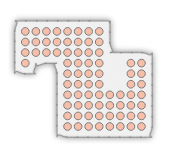
\includegraphics[width=5cm]{example_gilbert_border} }}%
    \qquad
    \subfloat[\centering ]{{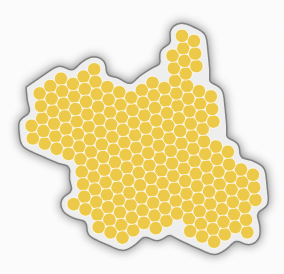
\includegraphics[width=5cm]{example_gosper_border} }}%
    \caption{(a) An example of Gilbert cluster border (b) An example of Gosper cluster borders}%
    \label{fig: borders}%
\end{figure}
\subparagraph{Labeling}
Labeling the clusters is essential for users to explore the dataset.
We use the topic assignment described in \autoref{sec: tag_assignment} to label the clusters.
When using SFC layouts, determining the label position automatically is challenging because the shape of the clusters can be irregular.
For a cluster, the label position is simply the centroid of the polygon.
When a cluster is expanded through user interaction, the sub-clusters within need to be clearly labeled as well.
Using the centroid of the sub-cluster as the label position is not a good choice because the label would cause a serious cluttering issue.
Therefore, for a sub-cluster, we first calculate the centroid of the sub-cluster, and then we extend the line from the parent cluster centroid to the sub-cluster centroid. 
Once the intersection point of the extended line and the parent border is found, we extend the line by a fixed amount to avoid any overlapping issues.
This results in a radial layout for the sub-cluster labels, as shown in~\autoref{fig: labels}.
The generalizability of the concave hull algorithm makes our labeling position calculation applicable to any curve we use for the SFC layout.
\begin{figure}%
    \centering
    \subfloat[\centering Label position of the cluster is the centroid of each cluster.]{{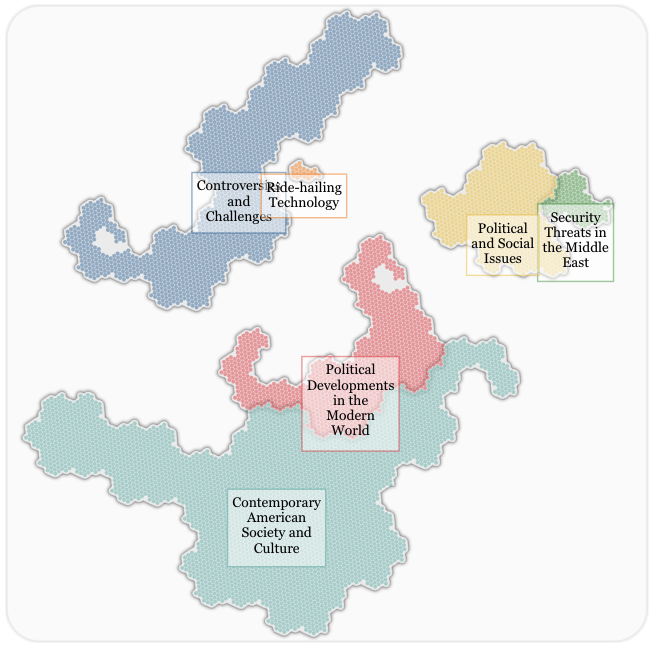
\includegraphics[width=0.5\columnwidth]{cluster_label} }}%
    \subfloat[\centering Labels of the sub-clusters of a cluster. The color indicates different sub-clusters. \label{fig: sub-cluster}]{{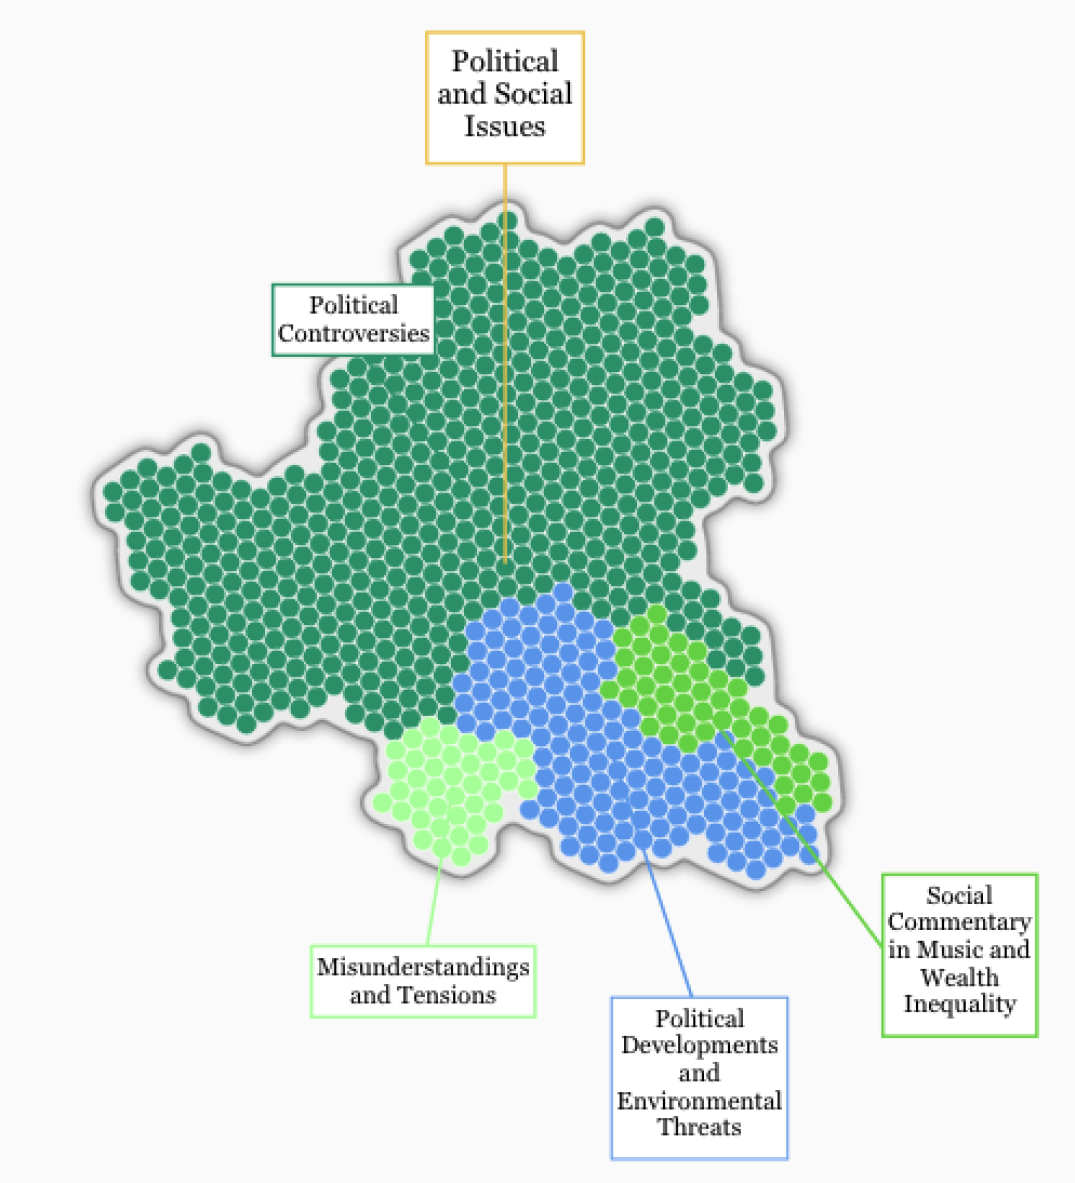
\includegraphics[width=0.5\columnwidth]{sub_cluster_label} }}%
    \qquad
    \subfloat[\centering Labels of the character cluster. The left part shows the categories of the characters as the cluster label. When documents are selected, the right part appears and shows the connected characters.\label{fig: character-cluster-label}]{{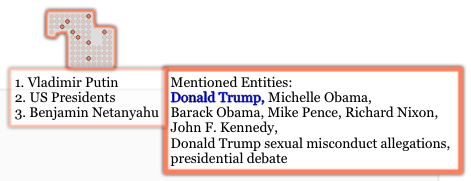
\includegraphics[width=5cm]{character_cluster_label} }}%
    \caption{(a) Labels (topics) of the document clusters (b) An example of expanded cluster labels (c) An example of character labels (categories) and highlighted characters}%
    \label{fig: labels}%
\end{figure}

% \subsection{Design Choices}
% \subparagraph{Why show all the nodes as circles}
% \subparagraph{Why hide the links}
